\documentclass{article}

%%%%
\usepackage[utf8]{inputenc}
\usepackage{longtable}
\usepackage{authblk}
\usepackage{adjustbox}

\usepackage{natbib}



\title{INDICE DE DESARROLLO (IDH) HUMANO POR DEPARTAMENTOS EN COLOMBIA}
% autores
\author[1]{\normalsize Juan Daniel Alvarez}



\affil[1]{\small  Departamento de Ingenieria Industrial,Universidad de los Andes\\
\texttt{{jd.alvarez17}@uniandes.edu.co}}


\date{29 de Junio de 2018}

\usepackage{Sweave}
\begin{document}
\Sconcordance{concordance:ProyectoFinal-JD.tex:ProyectoFinal-JD.Rnw:%
1 24 1 1 0 25 1 1 6 1 5 14 0 1 2 3 1 1 5 1 2 4 1 1 8 1 2 7 1 1 5 12 0 1 %
2 2 1 1 9 13 0 1 2 3 1 1 3 1 2 10 1 1 5 1 4 31 0 1 2 9 1 1 8 1 1 1 17 1 %
1 1 17 1 3 12 1}



\maketitle


\begin{abstract}
En este articulo se presentan los resultados de los diferentes analisis realizados a los valores de los indices de desarrollo humano que presentan los diferentes departamentos de Colombia, entre dichos analisis se incluyen exploracion univariada, bivariada, y espacial, ademas de una regresi<f3>n de los datos e histogramas de frecuencia de dichos valores. Utilizando los datos mencionados anteriormente y su respectivo analisis se determino cuales departamento presentan un indice de desarrollo humano alto, medio o bajo. Con el fin de entender un poco mas en cuales departamentos se presenta una situacion problematicoen relacion con el IDH en Colombia, con el fin de plantear soluciones al respecto. Adicinalmente, este trabajo se ha hecho bajo la filosofia del trabajo replicable y es un trabajo de exploracion y modelamineto de indices utilizando latex.

\end{abstract}

\section*{Introducción}

En este articulo se presentan los resultados a una investigacion realizada sobre el indice de desarrollo humano en Colombia. Colombia es un pais soberano situado en la region noroccidental de America del Sur, que se constituye en un estado unitario, social y democratico de derecho cuya forma de gobierno es presidencialista. Es una republica organizada politicamente en 32 departamentos descentralizados y el Distrito capital de Bogota, sede del gobierno nacional. Por otra parte, el Indice de Desarrollo Humano (IDH) se entiende como un indicador sintetico de los logros medios obtenidos en las dimensiones fundamentales del desarrollo humano, a saber, tener una vida larga y saludable, adquirir conocimientos y disfrutar de un nivel de vida digno. El IDH es la media aritmetica de los indices normalizados de cada una de las tres dimensiones.


Comencemos viendo que hay en la sección \ref{univariada} en la página \pageref{univariada}.

\clearpage


\section{Exploración Univariada}\label{univariada}

En esta sección realizo un analisis estadistico de los datos, obteniendo la siguiente tabla de referencia \ref{stats} para obtener un mejor analisis, en la cual analizamos las variables IDH, Poblacion cabecera y poblacion resto, obteniendo el numero de datos por variables y su mediana.


% Table created by stargazer v.5.2.2 by Marek Hlavac, Harvard University. E-mail: hlavac at fas.harvard.edu
% Date and time: vie., jun. 29, 2018 - 8:06:04 p. m.
\begin{table}[!htbp] \centering 
  \caption{Medidas estadisticas} 
  \label{stats} 
\begin{tabular}{@{\extracolsep{5pt}}lcc} 
\\[-1.8ex]\hline 
\hline \\[-1.8ex] 
Statistic & \multicolumn{1}{c}{N} & \multicolumn{1}{c}{Median} \\ 
\hline \\[-1.8ex] 
IDH & 32 & 0.804 \\ 
Poblacion.Cabecera & 32 & 717,197 \\ 
Poblacion.Resto & 32 & 268,111.5 \\ 
\hline \\[-1.8ex] 
\end{tabular} 
\end{table} 
En esta seccion realizo un analisis de las variables de interes de los datos, obteniendo los siguientes histogramas de referencia.

\begin{figure}[h]
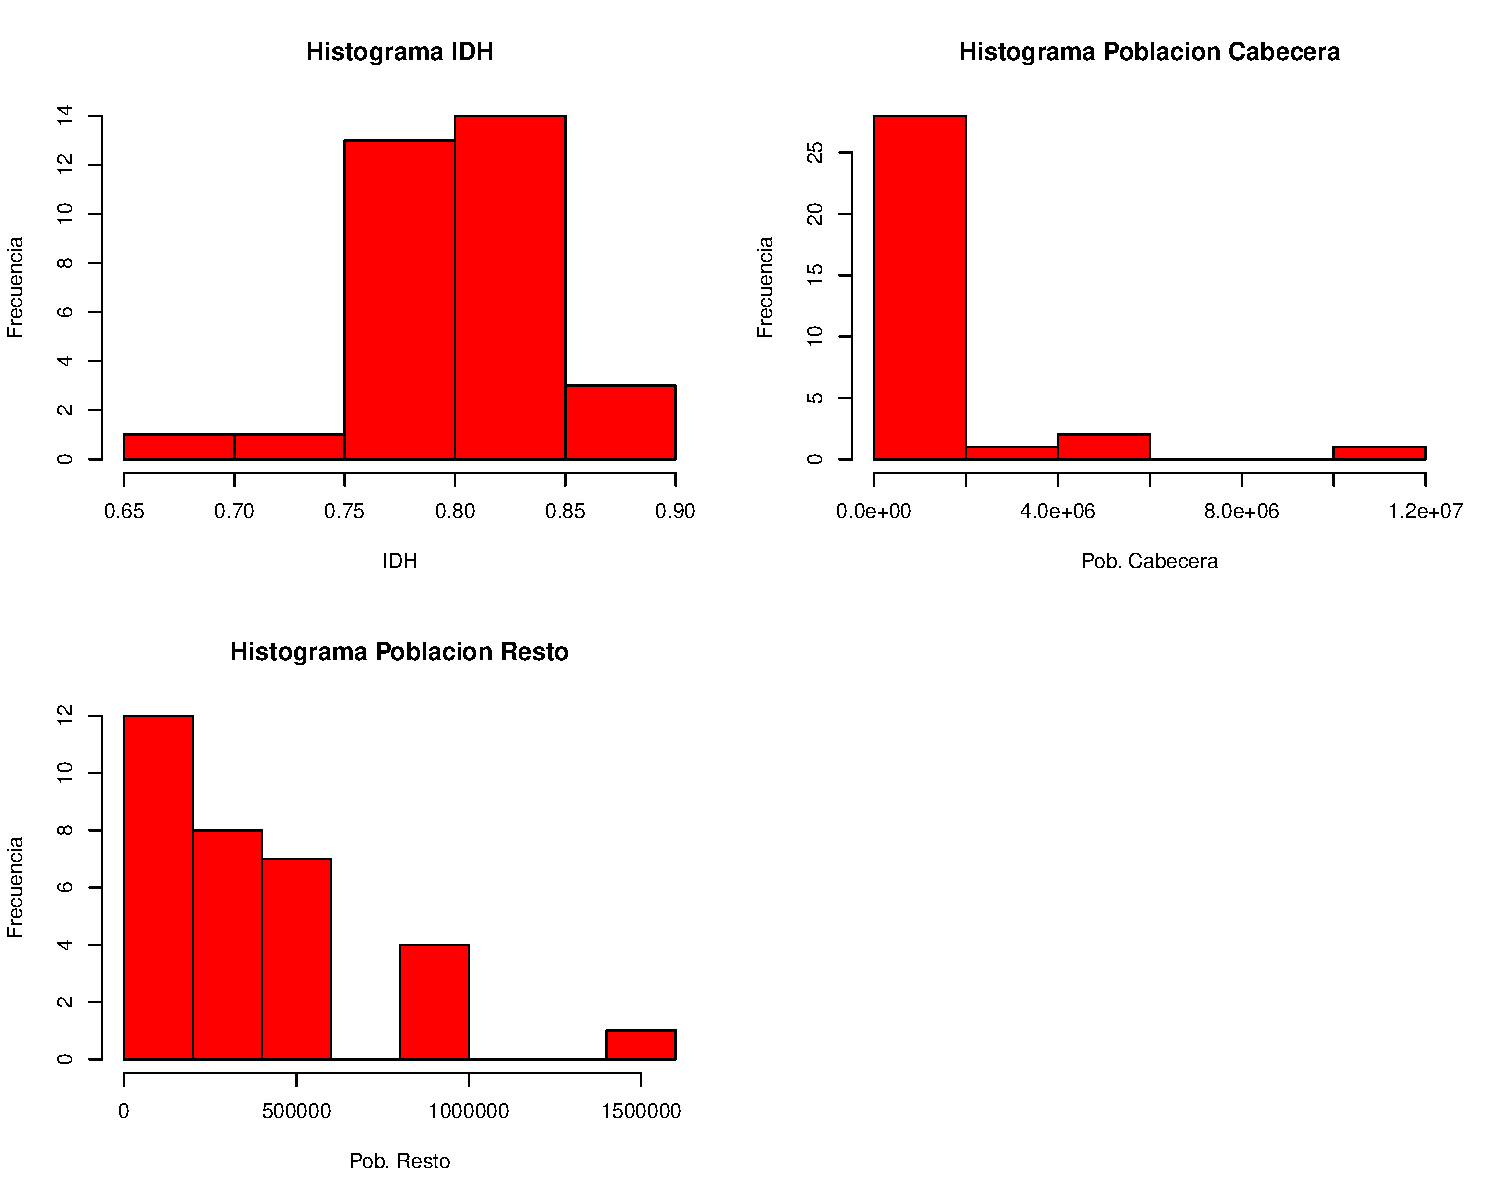
\includegraphics{ProyectoFinal-JD-hist1}
\caption{Histogramas}
\end{figure}

Teniendo en cuenta que los datos poblacionales pueden estar sesgados, se realiza una transformacion en los datos, con el fin de que estos se ajusten a la normalidad, obteniendo los siguientes histogramas.
\begin{figure}[h]
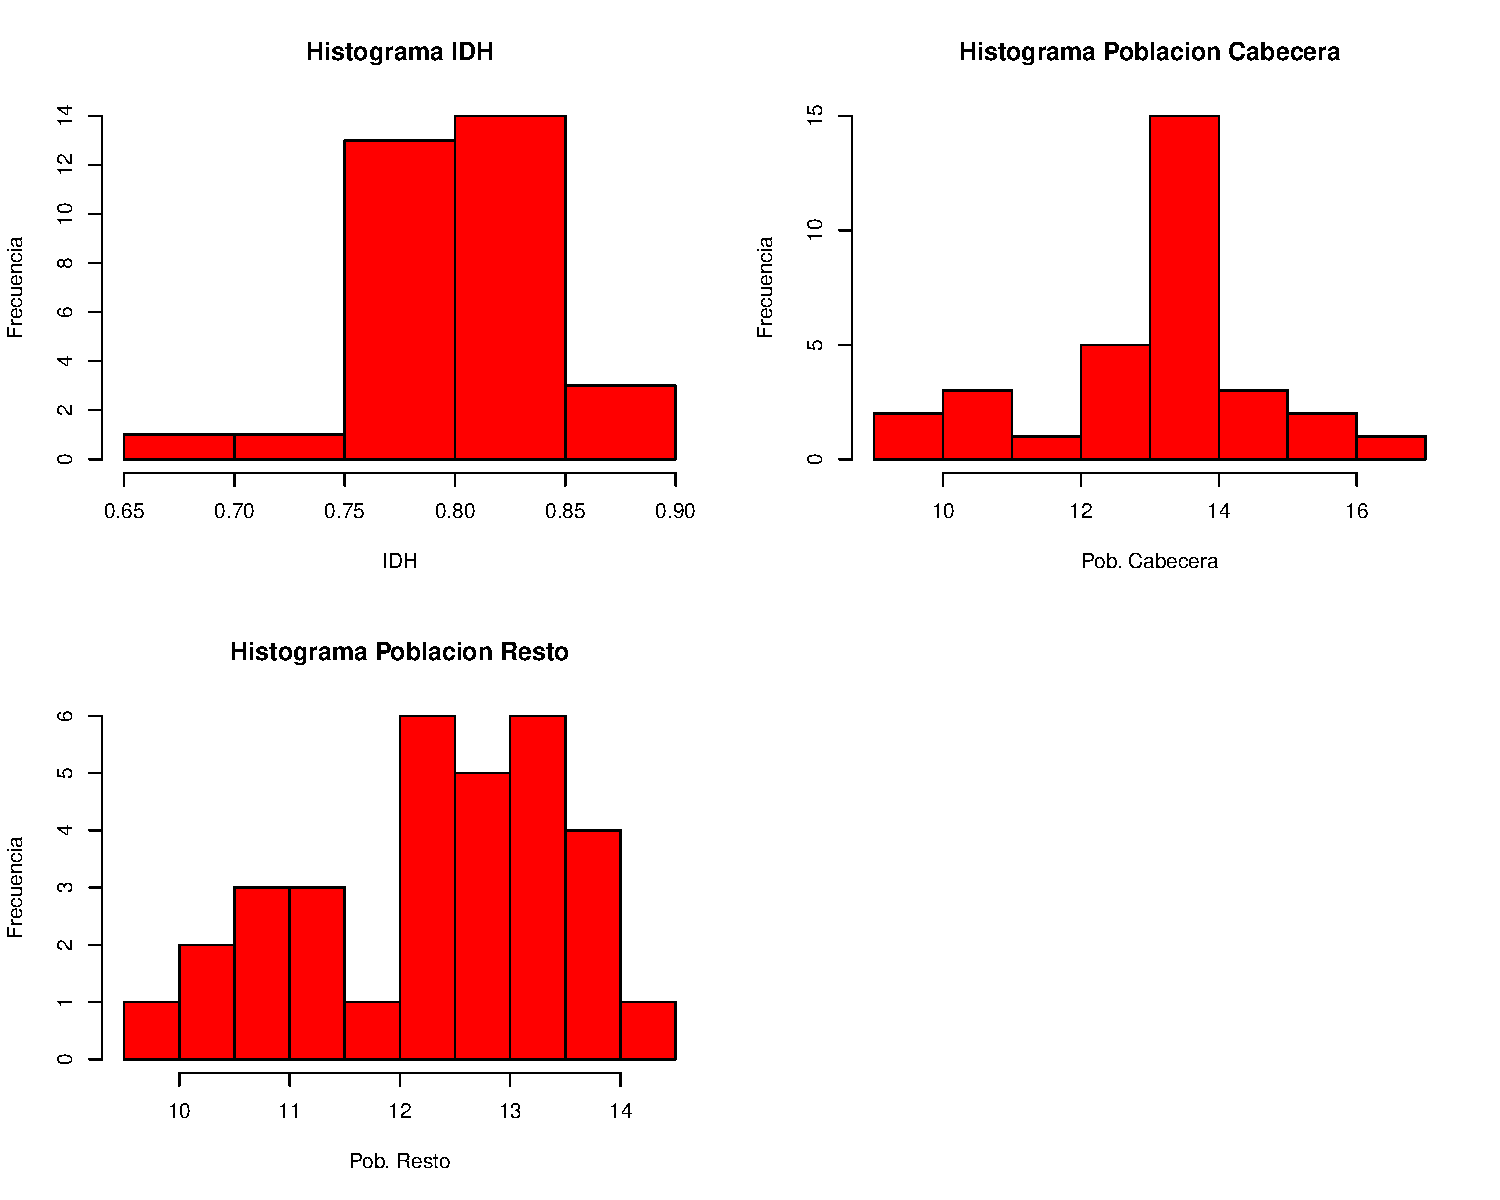
\includegraphics{ProyectoFinal-JD-hist2}
\caption{Histogramas normalizados}
\end{figure}
\clearpage
\section{Exploración Bivariada}

En este trabajo estamos interesados en el impacto de la pobacion en el IDH. Veamos las relaciones bivariadas que tiene esta variable con la mencionada anteriormente:


% Table created by stargazer v.5.2.2 by Marek Hlavac, Harvard University. E-mail: hlavac at fas.harvard.edu
% Date and time: vie., jun. 29, 2018 - 8:06:08 p. m.
\begin{table}[!htbp] \centering 
  \caption{Correlación del IDH con las poblaciones} 
  \label{corrDem} 
\begin{tabular}{@{\extracolsep{5pt}} cc} 
\\[-1.8ex]\hline 
\hline \\[-1.8ex] 
cabeLog & restoLog \\ 
\hline \\[-1.8ex] 
$0.487$ & $0.177$ \\ 
\hline \\[-1.8ex] 
\end{tabular} 
\end{table} 
Ahora, pasamos a ver la correlación entre las variables independientes:

% Table created by stargazer v.5.2.2 by Marek Hlavac, Harvard University. E-mail: hlavac at fas.harvard.edu
% Date and time: vie., jun. 29, 2018 - 8:06:08 p. m.
\begin{table}[!htbp] \centering 
  \caption{Correlación entre variables independientes} 
  \label{corrTableX} 
\begin{tabular}{@{\extracolsep{5pt}} ccc} 
\\[-1.8ex]\hline 
\hline \\[-1.8ex] 
 & cabeLog & restoLog \\ 
\hline \\[-1.8ex] 
cabeLog & 1 &  \\ 
restoLog & 0.84 & 1 \\ 
\hline \\[-1.8ex] 
\end{tabular} 
\end{table} 
Lo visto en la Tabla \ref{corrTableX} se refuerza claramente en la siguiente figura.
\begin{figure}[h]
\begin{adjustbox}{width=15cm,height=6cm}
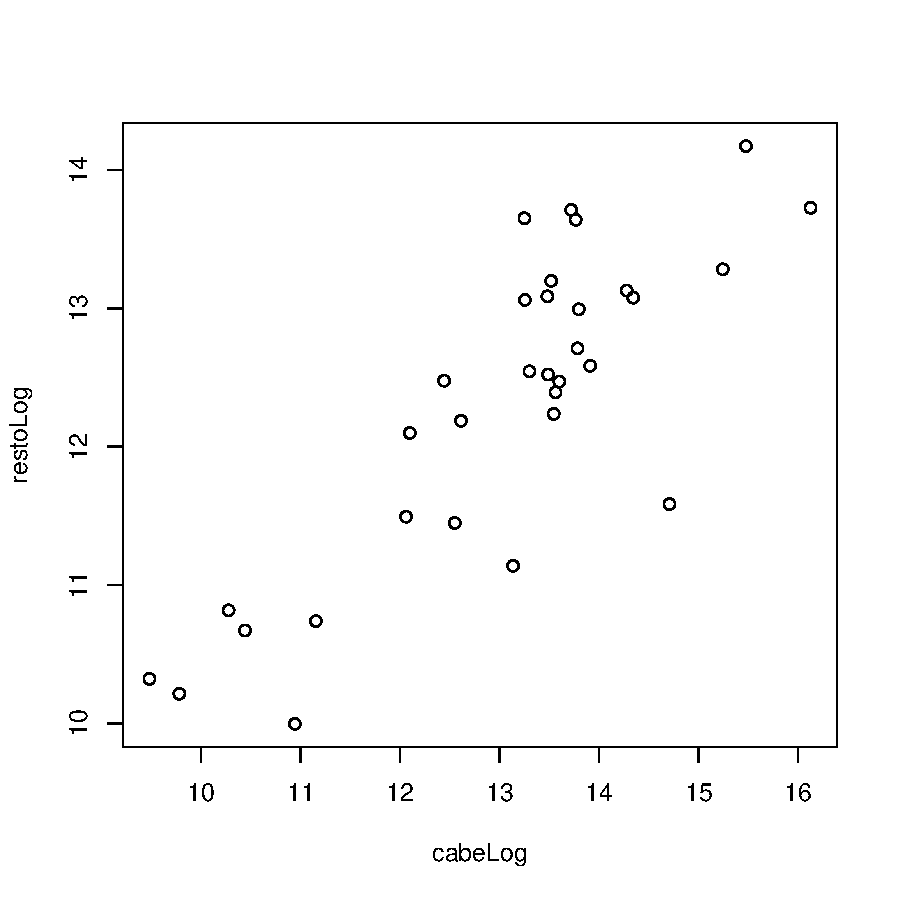
\includegraphics{ProyectoFinal-JD-corrPlot2}
\end{adjustbox}
\caption{Grafico de dispersion}
\end{figure}
\clearpage


\section{Modelos de Regresión}

Finalmente, vemos los modelos propuestos. Primero sin poblacion resto como independiente, y luego con está. Los resultados se muestran en la Tabla \ref{regresiones} de la página \pageref{regresiones}.



% Table created by stargazer v.5.2.2 by Marek Hlavac, Harvard University. E-mail: hlavac at fas.harvard.edu
% Date and time: vie., jun. 29, 2018 - 8:06:08 p. m.
\begin{table}[!htbp] \centering 
  \caption{Modelos de Regresion} 
  \label{regresiones} 
\begin{tabular}{@{\extracolsep{5pt}}lcc} 
\\[-1.8ex]\hline 
\hline \\[-1.8ex] 
 & \multicolumn{2}{c}{\textit{Dependent variable:}} \\ 
\cline{2-3} 
\\[-1.8ex] & \multicolumn{2}{c}{IDH} \\ 
\\[-1.8ex] & (1) & (2)\\ 
\hline \\[-1.8ex] 
 cabeLog & 0.013$^{***}$ & 0.031$^{***}$ \\ 
  & (0.004) & (0.007) \\ 
  & & \\ 
 restoLog &  & $-$0.030$^{***}$ \\ 
  &  & (0.010) \\ 
  & & \\ 
 Constant & 0.634$^{***}$ & 0.766$^{***}$ \\ 
  & (0.055) & (0.065) \\ 
  & & \\ 
\hline \\[-1.8ex] 
Observations & 32 & 32 \\ 
R$^{2}$ & 0.238 & 0.425 \\ 
Adjusted R$^{2}$ & 0.212 & 0.385 \\ 
Residual Std. Error & 0.037 (df = 30) & 0.033 (df = 29) \\ 
F Statistic & 9.347$^{***}$ (df = 1; 30) & 10.706$^{***}$ (df = 2; 29) \\ 
\hline 
\hline \\[-1.8ex] 
\textit{Note:}  & \multicolumn{2}{r}{$^{*}$p$<$0.1; $^{**}$p$<$0.05; $^{***}$p$<$0.01} \\ 
\end{tabular} 
\end{table} 
\clearpage


\section{Exploración Espacial}

Como acabamos de ver en la Tabla \ref{regresiones} en la página \pageref{regresiones}, si quisieras sintetizar la multidimensionalidad de nuestros indicadores se pueden utilizar los valores de IDH de las variables que tenemos. 

Asi, propongo que calculemos tres conglomerados de departamentos usando toda la información del IDH, de los mismo en Colombia. Este proceso de conglomeracion se puede lograr gracias a los descubrimientos y analisis propuestos por McQueen \cite{macqueen_methods_nodate}. Los tres conglomerados se muestran en la Figura \ref{clustmap}.




\begin{figure}[h]
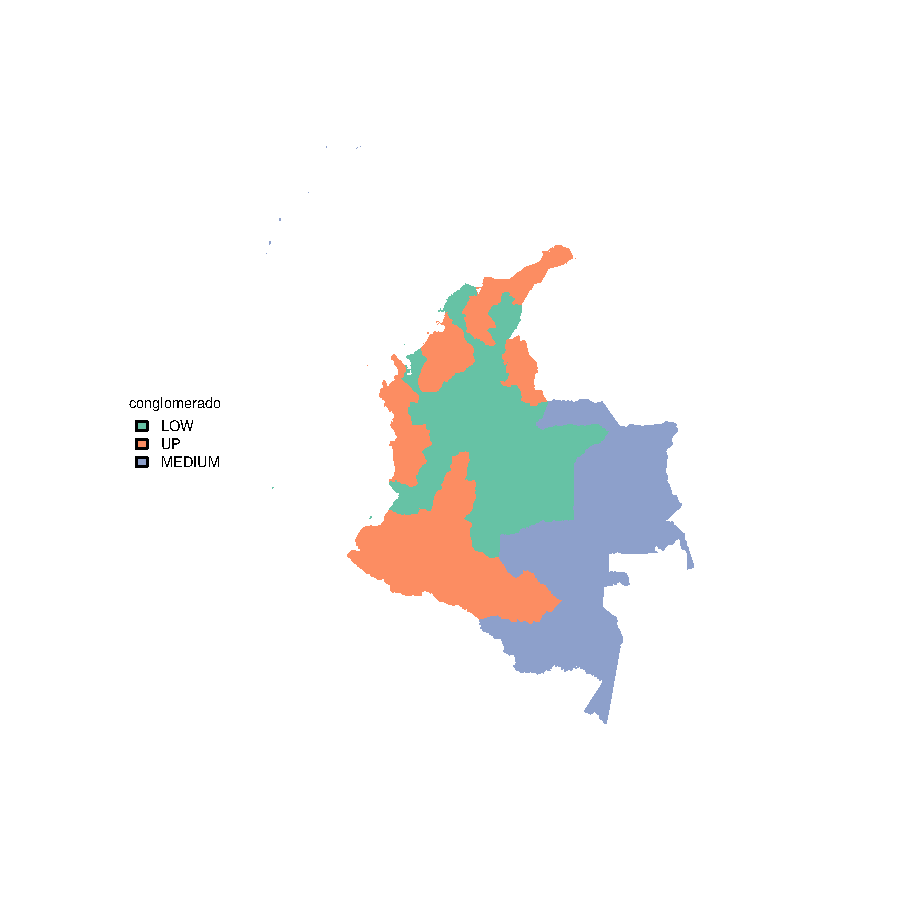
\includegraphics{ProyectoFinal-JD-plotMap1}

\caption{Departamentos conglomerados segun sus IDH}\label{clustmap}
\end{figure}
\clearpage


\bibliographystyle{abbrv}
\renewcommand{\refname}{Bibliografia}
\bibliography{PFINAL}



\end{document}
